\documentclass[frenchb]{beamer}
\usepackage[utf8]{inputenc}
\usepackage[T1]{fontenc}
\usepackage{babel}
\usepackage{listings}
\usepackage{verbatim}
\usepackage{fancyvrb}
\usepackage{color}


\setbeamercolor{haut}{fg=white,bg=darkgray}
\setbeamercolor{bas}{fg=black,bg=blue!5}
\lstset{% general command to set parameter(s)
basicstyle=\small,
% print whole listing small
keywordstyle=\color{green},
% underlined bold black keywords
identifierstyle=\color{darkgray},
% nothing happens
commentstyle=\color{white}, % white comments
stringstyle=\ttfamily,
% typewriter type for strings
showstringspaces=false}
% no special string spaces
	
\usetheme{CambridgeUS}
%\usetheme{Hannover}
%\usetheme{Singapore}	

\AtBeginSection[] {
  \begin{frame}<beamer>{}
    \tableofcontents[currentsection]
  \end{frame}
}

\title[M2GL-VET]{Simulateur de synthétiseur de son analogique}
\author{Maxime Simon\and Julien Richard-Foy\and Julien Névo \and Cyrille Folliot}
\institute[ISTIC]{Université de Rennes 1}
\begin{document}

\begin{frame}
    \titlepage
\end{frame}
	
	
\begin{frame}{Plan de l'intervention}
    \tableofcontents
\end{frame}


\section{Introduction}


\begin{frame}{Un objectif}
    \begin{figure}
        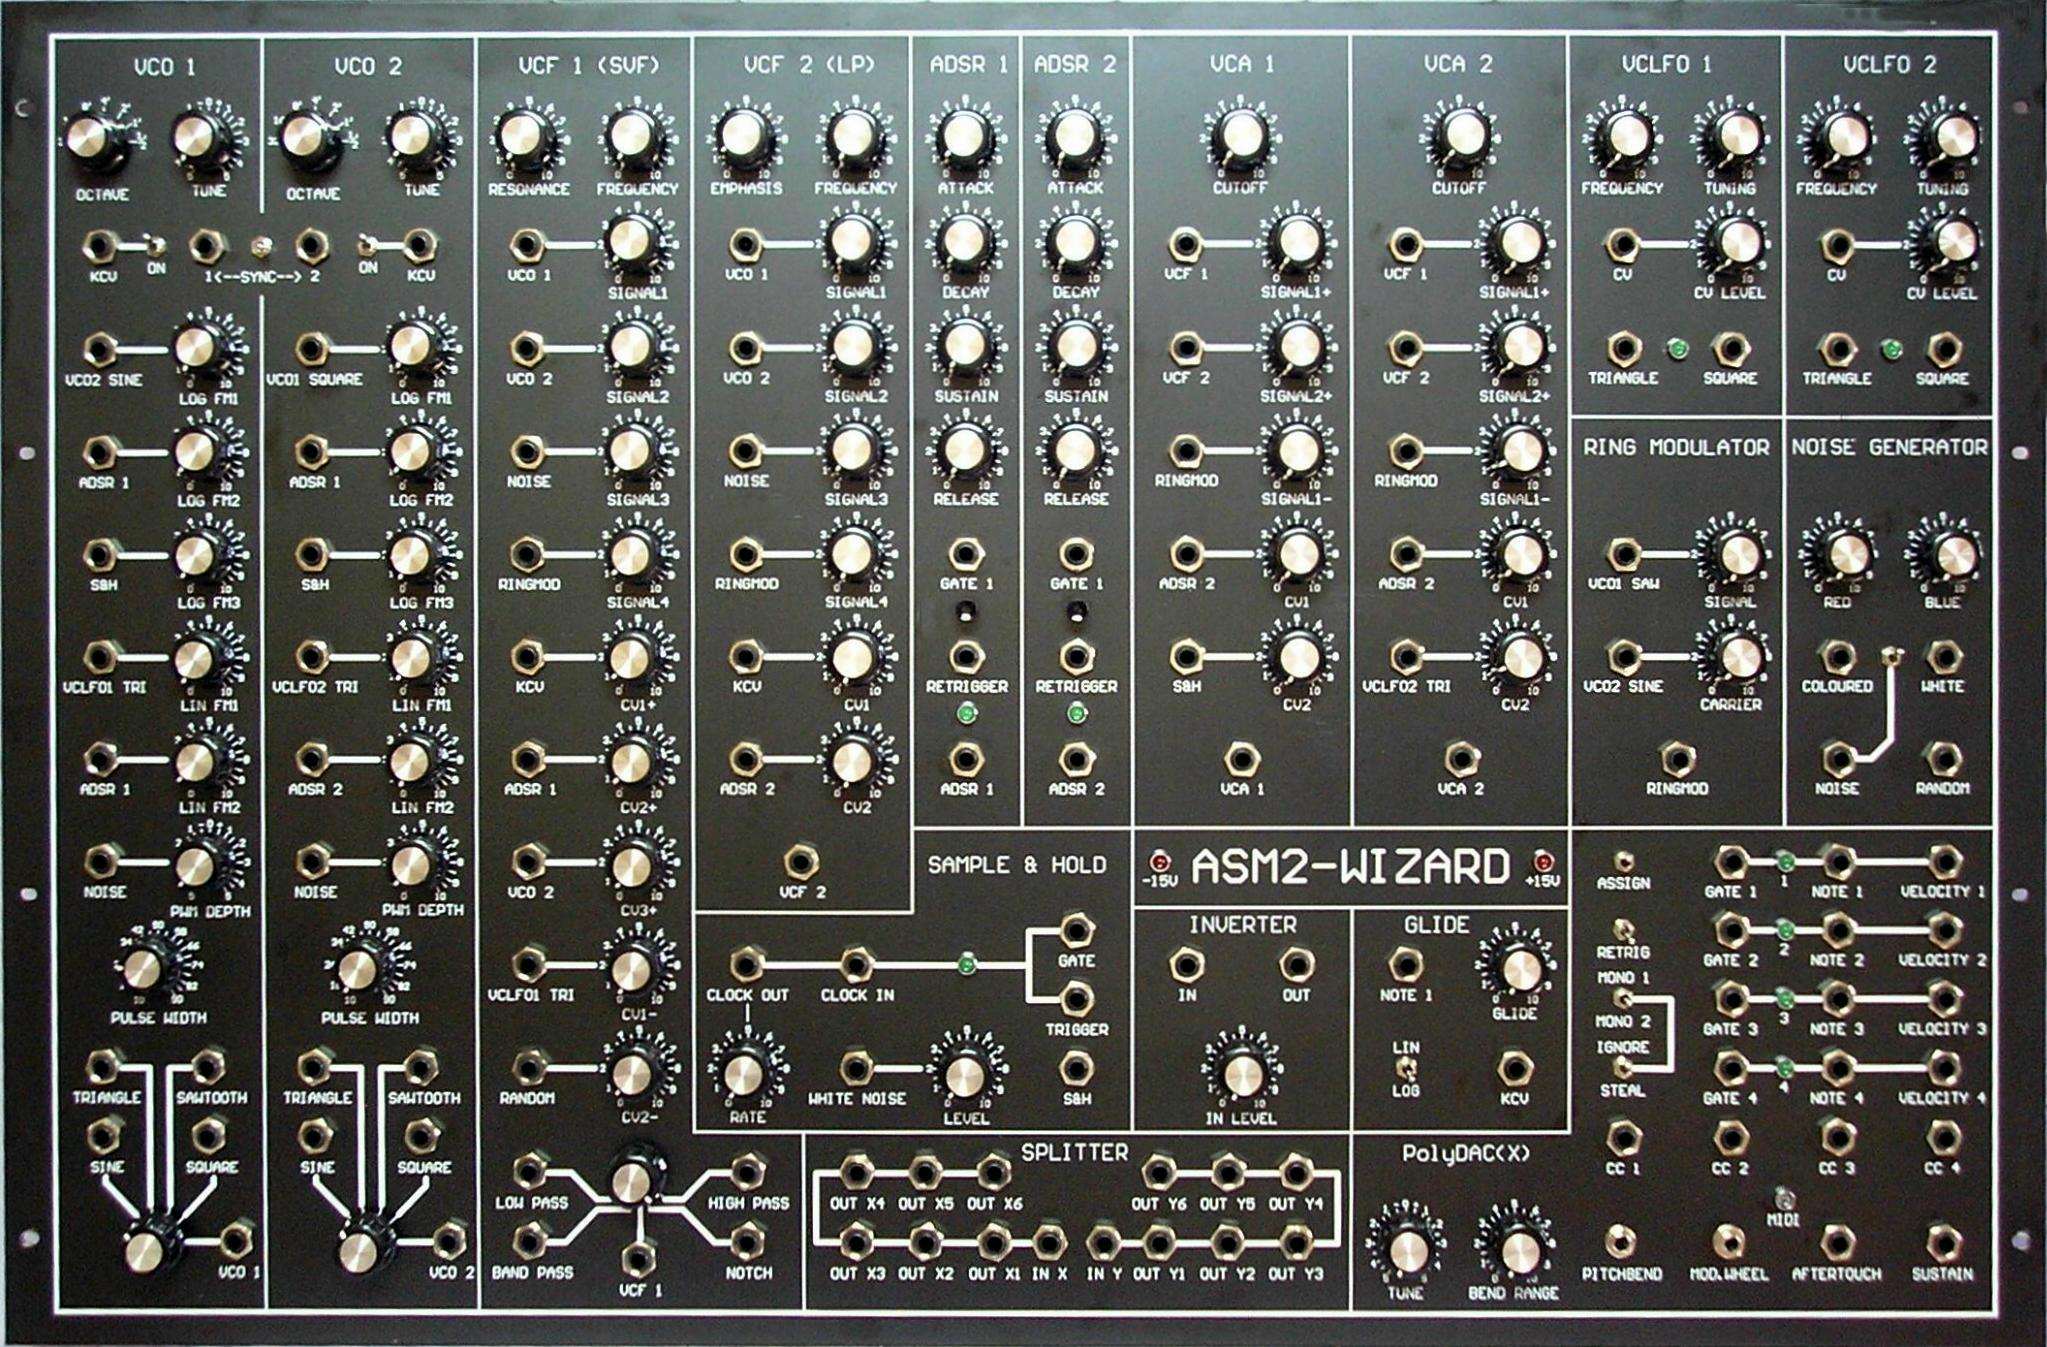
\includegraphics[width=8cm ]{../img/png/synth.jpg}
    \end{figure}
\end{frame}
\begin{frame}{Une équipe}
    \begin{columns}
        \begin{column}[l]{7cm}
            \begin{figure}
                
\includegraphics[width=6cm ]{../img/png/back.jpg}
            \end{figure}
        \end{column}
    \begin{column}[l]{9cm}
    \begin{itemize}  
        \item Julien Névo\\\tiny{Responsable projet}\normalsize
        \item Julien Richard-Foy\\\tiny{Responsable conception}\normalsize
        \item Maxime Simon\\\tiny{Responsable tests}\normalsize
        \item Cyrille Folliot\\\tiny{Responsable documentation}\normalsize
    \end{itemize}
    \end{column}
    \end{columns}
\end{frame}

\begin{frame}{Une organisation du travail liée au modèle PAC}
 \begin{columns}[t]
  \begin{column}{5cm}
  \begin{block}{Code métier~: Julien \& Cyrille}
             \begin{itemize}
                \item Moteur audio
                \item Modules du synthétiseur
            \end{itemize}    
  \end{block} 
  \end{column}
  
  \begin{column}{5cm}
  \begin{block}{IHM~: Maxime \& Julien}
            \begin{itemize}
                \item Contrôles PAC
                \item Présentations PAC
            \end{itemize}
  \end{block}   
  \end{column}
 \end{columns}  
\end{frame}

\begin{frame}{Le choix d'un développement itératif}

\begin{block}{Trois grandes étapes~:}
\begin{itemize}
    \item Construction du modèle de l'application : PIM \& PSM
    \item Développement itératif
    \item Debuggage, optimisation, documentation externe
\end{itemize}
\end{block}
\end{frame}

\section{Conception}

\begin{frame}{Conception -- PIM -- Abstraction}
    \begin{figure}
        \includegraphics[height=7cm ]{../img/ps/business-pim-part1-1.pdf}
    \end{figure}
\end{frame}

\begin{frame}{Conception -- PIM -- Abstraction}
    \begin{figure}
        \includegraphics[height=7cm ]{../img/ps/business-pim-part1-2.pdf}
    \end{figure}
\end{frame}

\begin{frame}{Conception -- PIM -- Abstraction}
    \begin{figure}
        \includegraphics[height=7cm ]{../img/ps/business-pim-part1-3.pdf}
    \end{figure}
\end{frame}

\begin{frame}{Conception -- PIM -- Abstraction}
    \begin{figure}
        \includegraphics[height=7cm ]{../img/ps/business-pim-part1-4.pdf}
    \end{figure}
\end{frame}

\begin{frame}{Conception -- PIM -- Abstraction}
    \begin{figure}
        \includegraphics[width=12cm ]{../img/ps/business-pim-part2-1.pdf}
    \end{figure}
\end{frame}

\begin{frame}{Conception -- PIM -- Abstraction}
    \begin{figure}
        \includegraphics[width=12cm ]{../img/ps/business-pim-part2-2.pdf}
    \end{figure}
\end{frame}

\begin{frame}{Conception -- PIM -- Abstraction}
    \begin{figure}
        \includegraphics[width=12cm ]{../img/ps/business-pim-part2-3.pdf}
    \end{figure}
\end{frame}

\begin{frame}{Conception -- PIM -- Abstraction}
    \begin{figure}
        \includegraphics[width=12cm ]{../img/ps/business-pim-part2-4.pdf}
    \end{figure}
\end{frame}

\begin{frame}{Conception -- PIM -- Abstraction}
    \begin{figure}
        \includegraphics[width=12cm ]{../img/ps/business-pim-part2-5.pdf}
    \end{figure}
\end{frame}

\begin{frame}{Conception -- PIM -- Interface utilisateur}
    \begin{figure}
        \includegraphics[height=7cm]{../img/ps/pacdimmer-pim.pdf}
    \end{figure}
\end{frame}

\begin{frame}{Le choix d'un langage et d'un framework}
    \pause
    \begin{columns}
        \begin{column}[l]{5cm}
            \begin{block}{Langage}
            \begin{center}
                \includegraphics[width=2cm]{../img/ps/C_plus_plus.pdf}
            \end{center}
            \begin{itemize}
                \item Performance
            \end{itemize}
            \end{block}
        \end{column}
        \pause
        \begin{column}[r]{5cm}
            \begin{block}{Framework}
            \begin{center}
                \includegraphics[width=2cm]{../img/ps/Qt.pdf}
            \end{center}
            \begin{itemize}
                \item API Élégante
                \item \textit{Full featured}
                \item «~Meta Object~»
            \end{itemize}
            \end{block}
        \end{column}
    \end{columns}
\end{frame}

\section{Tests}

\begin{frame}{Plan de tests et résultats}
    \begin{block}{Plop}
        \begin{itemize}
            \item Tests unitaires
            \item Tests fonctionnels
            \item Développement de mocks
        \end{itemize}
    \end{block}

    \begin{block}{Qualité}
        Hook pre-commit
    \end{block}
\end{frame}

\section{Documentation}

\begin{frame}{Preview documentation interne et externe}
    \begin{itemize}
        \item Doxygen
        \item Manuel utilisateur
    \end{itemize}
\end{frame}

\section{Démonstration}

\begin{frame}{Que le spectacle commence !}
    \begin{center}
        Démonstration
    \end{center}
\end{frame}

\section{Synthèse sur l’expérience}

\begin{frame}{Problèmes rencontrés}
    \begin{center}
        \includegraphics[width=7cm]{../img/ps/pacmodule-psm.pdf}
    \end{center}
    \pause
    \begin{columns}
        \begin{column}[l]{7cm}
        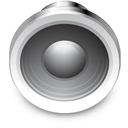
\includegraphics[width=3cm]{../img/png/arts128x128.png}
        \end{column}
        \pause
        \begin{column}[r]{4cm}
        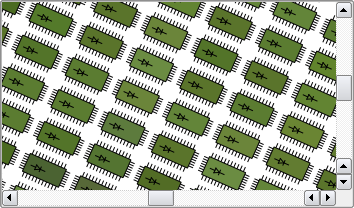
\includegraphics[width=3cm]{../img/png/graphicsview-view.png}
        \end{column}
    \end{columns}
\end{frame}

\end{document}
